\section{二代测序数据分析}

\subsection{常见术语}
\begin{frame}
  \frametitle{NGS | 数据分析 | 术语 | \textcolor{red}{深度 vs. 覆盖度}}
  \begin{block}{深度(depth)}
    \begin{itemize}
      \item 也叫乘数,衡量测序量的首要参数;测序得到的总碱基数与待测基因组大小的比值;每个碱基被测序的平均次数
      \item 假设一个基因大小为2M,测序获得的总数据量为20M,那么深度为10X
    \end{itemize}
  \end{block}
  \pause
  \begin{block}{覆盖度(coverage)}
    \begin{itemize}
      \item 测序获得的序列占整个捕获区域/基因组的比例
      \item 由于基因组中的高GC、重复序列等复杂结构的存在,测序最终拼接组装获得的序列往往无法覆盖所有的区域,这部分没有获得的区域就称为Gap。例如一个细菌基因组测序,覆盖度是98\%,那么还有2\%的序列区域是没有通过测序获得的。
    \end{itemize}
  \end{block}
\end{frame}

\begin{frame}
  \frametitle{NGS | 数据分析 | 术语 | 深度 vs. 覆盖度}
  \begin{block}{实验}
对长100bp的目标区域进行捕获测序:采用单端测序,每个read长5bp;总共得到了200个reads;把所有的reads比对到目标区域后,100bp的目标区域中有98bp的位置至少有1个read覆盖到,换言之,剩余的2bp没有任何reads覆盖。
  \end{block}
  \pause
  \begin{block}{深度与覆盖度}
    \begin{itemize}
      \item 深度:$200 \times 5 / 100 = 10$
      \item 覆盖度:$98 / 100 \times 100\% = 98\%$
    \end{itemize}
  \end{block}
\end{frame}

\begin{frame}
  \frametitle{NGS | 数据分析 | 术语 | 深度 vs. 覆盖度}
  \begin{figure}
    \centering
    \includegraphics[width=0.85\textwidth]{c2_genomics/term_depth_cov_01.png}
  \end{figure}
\end{frame}

\begin{frame}
  \frametitle{NGS | 数据分析 | 术语 | SE vs. PE}
  \begin{figure}
    \centering
    \includegraphics[width=0.85\textwidth]{c2_genomics/term_se_pe_01.jpg}
  \end{figure}
\end{frame}

\begin{frame}
  \frametitle{NGS | 数据分析 | 术语 | PE}
  \begin{block}{Paired-End Sequencing}
    \begin{itemize}
      \item allows users to sequence both ends of a fragment and generate high-quality, alignable sequence data
      \item facilitates detection of genomic rearrangements and repetitive sequence elements, as well as gene fusions and novel transcripts
    \end{itemize}
  \end{block}
  \begin{figure}
    \centering
    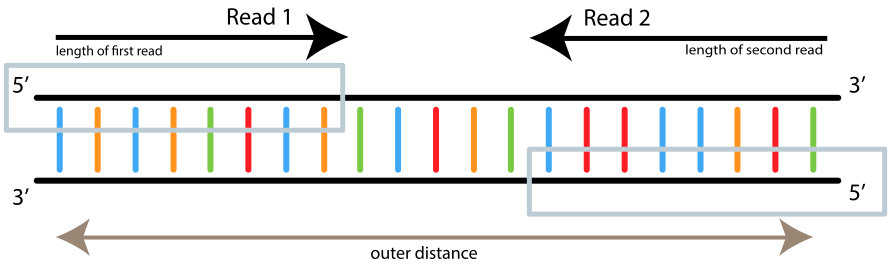
\includegraphics[width=0.9\textwidth]{c2_genomics/term_pe_01.png}
  \end{figure}
\end{frame}

\begin{frame}
  \frametitle{NGS | 数据分析 | 术语 | PE}
  \begin{figure}
    \centering
    \includegraphics[width=0.85\textwidth]{c2_genomics/term_pe_03.png}\\
    \vspace{1em}
    \includegraphics[width=0.85\textwidth]{c2_genomics/term_se_pe_04.png}
  \end{figure}
\end{frame}

\begin{frame}
  \frametitle{NGS | 数据分析 | 术语 | \textcolor{red}{PE}}
  \begin{figure}
    \centering
    \only<1->{\includegraphics[width=\textwidth]{c2_genomics/term_insert_size_01.png}}\\
    \vspace{1em}
    \only<2->{\includegraphics[width=\textwidth]{c2_genomics/term_insert_size_02.png}}
  \end{figure}
  \only<3->{
  \begin{block}{Conclusion}
    Remember that ``\textcolor{red}{insert}" refers to the DNA fragment between the adaptors, and not the gap between R1 and R2. Instead we refer to that as the ``\textcolor{red}{inner mate distance}".
  \end{block}
  }
\end{frame}

\begin{frame}
  \frametitle{NGS | 数据分析 | 术语 | PE}
  \begin{figure}
    \centering
    \includegraphics[width=0.85\textwidth]{c2_genomics/term_pe_02.png}
  \end{figure}
\end{frame}

\begin{frame}
  \frametitle{NGS | 数据分析 | 术语 | 其他}
  \begin{figure}
    \centering
    \includegraphics[width=\textwidth]{c2_genomics/term_other_01.png}
  \end{figure}
\end{frame}

\subsection{分析流程}
\begin{frame}
  \frametitle{NGS | 数据分析 | 流程 | 概述 | 总览}
  \begin{figure}
    \centering
    \includegraphics[width=\textwidth]{c2_genomics/workflow_ngs_05.png}
  \end{figure}
\end{frame}

\begin{frame}
  \frametitle{NGS | 数据分析 | 流程 | 概述 | 总览}
  \begin{figure}
    \centering
    \includegraphics[width=0.85\textwidth]{c2_genomics/workflow_ngs_10.png}
  \end{figure}
\end{frame}

\begin{frame}
  \frametitle{NGS | 数据分析 | 流程 | 概述 | \textcolor{red}{Seqs}}
  \begin{figure}
    \centering
    \includegraphics[width=0.9\textwidth]{c2_genomics/workflow_ngs_03.png}
  \end{figure}
\end{frame}

\begin{frame}
  \frametitle{NGS | 数据分析 | 流程 | 概述 | Seqs}
  \begin{figure}
    \centering
    \includegraphics[width=\textwidth]{c2_genomics/workflow_ngs_04.png}
  \end{figure}
\end{frame}

\begin{frame}
  \frametitle{NGS | 数据分析 | 流程 | 概述 | \textcolor{red}{WES}}
  \begin{figure}
    \centering
    \includegraphics[width=0.6\textwidth]{c2_genomics/workflow_exome_05.png}
  \end{figure}
\end{frame}

\begin{frame}
  \frametitle{NGS | 数据分析 | 流程 | 概述 | \textcolor{red}{WES}}
  \begin{figure}
    \centering
    \includegraphics[width=0.9\textwidth]{c2_genomics/workflow_exome_03.png}
  \end{figure}
\end{frame}

\begin{frame}
  \frametitle{NGS | 数据分析 | 流程 | 质控(QC)}
  \begin{figure}
    \centering
    \includegraphics[width=0.9\textwidth]{c2_genomics/qc_pre_04.png}
  \end{figure}
\end{frame}

\begin{frame}
  \frametitle{NGS | 数据分析 | 流程 | 质控}
  \begin{figure}
    \centering
    \includegraphics[width=0.9\textwidth]{c2_genomics/qc_report_01.png}
  \end{figure}
\end{frame}

\begin{frame}
  \frametitle{NGS | 数据分析 | 流程 | 质控 | 工具}
  \begin{figure}
    \centering
    \includegraphics[width=\textwidth]{c2_genomics/qc_tool_01.png}
  \end{figure}
\end{frame}

\begin{frame}
  \frametitle{NGS | 数据分析 | 流程 | 质控 | \textcolor{red}{工具}}
  \begin{block}{FastQC}
    A quality control tool for high throughput sequence data.
  \end{block}
  \vspace{-0.2em}
  \pause
  \begin{block}{NGS QC Toolkit}
    A toolkit for the quality control (QC) of next generation sequencing (NGS) data.
  \end{block}
  \vspace{-0.2em}
  \pause
  \begin{block}{AfterQC}
    Automatic Filtering, Trimming, Error Removing and Quality Control for fastq data.
  \end{block}
  \vspace{-0.2em}
  \pause
  \begin{block}{Others}
    \begin{itemize}
      \item SolexaQA: calculates sequence quality statistics and creates visual representations of data quality for second-generation sequencing data.
      \item ...
    \end{itemize}
  \end{block}
\end{frame}

\begin{frame}
  \frametitle{NGS | 数据分析 | 流程 | 质控 | FastQC}
  \begin{figure}
    \centering
    \includegraphics[width=0.9\textwidth]{c2_genomics/qc_fastqc_00.png}
  \end{figure}
\end{frame}

\begin{frame}
  \frametitle{NGS | 数据分析 | 流程 | 预处理}
  \begin{block}{目的}
 manipulating the sequences to produce better mapping results
  \end{block}
  \pause
  \begin{block}{内容}
    \begin{itemize}
      \item Collapser: Collapsing identical sequences into a single sequence
      \item Clipper: Removing sequencing adapters/linkers
      \item Splitter: Splitting barcode containning multiple samples
      \item Filter: Filters sequences based on quality
      \item Trimmer: Trims (cuts) sequences based on quality
      \item Formatter: Rename identifiers, Reverse-complement, Mask nucleotides, Convert RNA $\leftrightarrow$ DNA, ...
      \item ...
    \end{itemize}
  \end{block}
\end{frame}

\begin{frame}
  \frametitle{NGS | 数据分析 | 流程 | 预处理}
  \begin{figure}
    \centering
    \includegraphics[width=0.9\textwidth]{c2_genomics/pre_02.png}
  \end{figure}
\end{frame}

\begin{frame}
  \frametitle{NGS | 数据分析 | 流程 | 预处理 | \textcolor{red}{工具}}
  \begin{block}{FASTX-Toolkit}
    A collection of command line tools for Short-Reads FASTA/FASTQ files preprocessing.
  \end{block}
  \pause
  \begin{block}{PRINSEQ}
    PReprocessing and INformation of SEQuence data. A publicly available tool that is able to filter, reformat and trim your sequences and to provide you summary statistics for your sequence data.
  \end{block}
  \pause
  \begin{block}{cutadapt}
    Cutadapt finds and removes adapter sequences, primers, poly-A tails and other types of unwanted sequence from your high-throughput sequencing reads. It can also modify and filter reads in various ways.
  \end{block}
\end{frame}

\begin{frame}
  \frametitle{NGS | 数据分析 | 流程 | 预处理 | FASTX-Toolkit}
  \begin{figure}
    \centering
    \includegraphics[width=0.58\textwidth]{c2_genomics/pre_fastx_cli_01.png}
    \includegraphics[width=0.4\textwidth]{c2_genomics/pre_fastx_galaxy_01.png}
  \end{figure}
\end{frame}

\begin{frame}
  \frametitle{NGS | 数据分析 | 流程 | 比对}
  \begin{figure}
    \centering
    \includegraphics[width=0.9\textwidth]{c2_genomics/mapping_01.png}
  \end{figure}
\end{frame}

\begin{frame}
  \frametitle{NGS | 数据分析 | 流程 | 比对}
  \begin{figure}
    \centering
    \includegraphics[width=0.9\textwidth]{c2_genomics/mapping_07.png}
  \end{figure}
\end{frame}

\begin{frame}
  \frametitle{NGS | 数据分析 | 流程 | 比对 | 算法}
  \begin{figure}
    \centering
    \includegraphics[width=0.65\textwidth]{c2_genomics/mapping_11.png}
  \end{figure}
\end{frame}

\begin{frame}
  \frametitle{NGS | 数据分析 | 流程 | 比对 | 工具}
  \begin{figure}
    \centering
    \includegraphics[width=0.9\textwidth]{c2_genomics/tool_alignment_02.png}
  \end{figure}
\end{frame}

\begin{frame}
  \frametitle{NGS | 数据分析 | 流程 | 比对 | 工具}
  \begin{figure}
    \centering
    \includegraphics[width=0.9\textwidth]{c2_genomics/tool_alignment_03.png}
  \end{figure}
\end{frame}

\begin{frame}
  \frametitle{NGS | 数据分析 | 流程 | 比对 | 工具}
  \begin{figure}
    \centering
    \includegraphics[width=0.8\textwidth]{c2_genomics/tool_alignment_04.png}
  \end{figure}
\end{frame}

\begin{frame}
  \frametitle{NGS | 数据分析 | 流程 | 比对 | 工具}
  \begin{figure}
    \centering
    \includegraphics[width=0.9\textwidth]{c2_genomics/tool_alignment_01.png}
  \end{figure}
\end{frame}

\begin{frame}
  \frametitle{NGS | 数据分析 | 流程 | 比对 | \textcolor{red}{工具}}
  \begin{block}{BWA}
    BWA(Burrows-Wheeler Aligner) is a software package for mapping low-divergent sequences against a large reference genome, such as the human genome.
  \end{block}
  \pause
  \begin{block}{Bowtie}
    \begin{itemize}
      \item Bowtie is an ultrafast, memory-efficient short read aligner.
      \item Bowtie 2 is an ultrafast and memory-efficient tool for aligning sequencing reads to long reference sequences.
    \end{itemize}
  \end{block}
\end{frame}

\begin{frame}
  \frametitle{NGS | 数据分析 | 流程 | 比对 | \textcolor{red}{工具}}
  \begin{block}{SOAP}
    SOAP has been in evolution from a single alignment tool to a tool package that provides full solution to next generation sequencing data analysis.
    \begin{itemize}
      \item SOAPaligner/soap2: new alignment tool
      \item SOAPsnp: re-sequencing consensus sequence builder
      \item SOAPindel: indel finder
      \item SOAPsv: structural variation scanner
      \item SOAPdenovo: \textit{de novo} shot reads assembler
      \item SOAP3/GPU: GPU-accelerated alignment tool
    \end{itemize}
  \end{block}
\end{frame}

\begin{frame}
  \frametitle{NGS | 数据分析 | 流程 | 提取变异}
  \begin{figure}
    \centering
    \includegraphics[width=0.9\textwidth]{c2_genomics/snp_calling_01.jpg}
  \end{figure}
\end{frame}

\begin{frame}
  \frametitle{NGS | 数据分析 | 流程 | 提取变异 | \textcolor{red}{工具}}
  \begin{block}{SAMtools}
    SAMtools is a suite of programs for interacting with high-throughput sequencing data.
  \end{block}
  \pause
  \begin{block}{GATK}
    Genome Analysis Toolkit: Variant Discovery in High-Throughput Sequencing Data.\\
    The GATK toolkit offers a wide variety of tools with a primary focus on variant discovery and genotyping.
  \end{block}
  \pause
  \begin{block}{VarScan}
    VarScan is a platform-independent software tool developed at the Genome Institute at Washington University to detect variants in NGS data.
  \end{block}
\end{frame}

\begin{frame}
  \frametitle{NGS | 数据分析 | 流程 | 提取变异 | SAMtools}
  \begin{block}{SAMtools}
    SAMtools consists of three separate repositories:
    \begin{description}
      \item[SAMtools] Reading/writing/editing/indexing/viewing SAM/BAM/CRAM format
      \item[BCFtools] Reading/writing BCF2/VCF/gVCF files and calling/filtering/summarising SNP and short indel sequence variants
      \item[HTSlib] A C library for reading/writing high-throughput sequencing data
    \end{description}
  \end{block}
\end{frame}

\begin{frame}
  \frametitle{NGS | 数据分析 | 流程 | 提取变异 | GATK}
  \begin{figure}
    \centering
    \includegraphics[width=0.9\textwidth]{c2_genomics/snp_calling_gatk_01.png}\\
    \vspace{1em}
    \includegraphics[width=0.9\textwidth]{c2_genomics/snp_calling_gatk_02.png}
  \end{figure}
\end{frame}

\begin{frame}
  \frametitle{NGS | 数据分析 | 流程 | 注释变异 | \textcolor{red}{工具}}
  \begin{block}{SnpEff}
    Genetic variant annotation and effect prediction toolbox. It annotates and predicts the effects of variants on genes (such as amino acid changes).
  \end{block}
  \pause
  \begin{block}{ANNOVAR}
    ANNOVAR is an efficient software tool to utilize update-to-date information to functionally annotate genetic variants detected from diverse genomes (including human genome hg18, hg19, hg38, as well as mouse, worm, fly, yeast and many others).
  \end{block}
\end{frame}

\begin{frame}
  \frametitle{NGS | 数据分析 | 流程 | 注释变异 | \textcolor{red}{工具}}
  \begin{block}{VEP}
    VEP (Variant Effect Predictor) determines the effect of your variants (SNPs, insertions, deletions, CNVs or structural variants) on genes, transcripts, and protein sequence, as well as regulatory regions.
  \end{block}
  \pause
  \begin{block}{SeattleSeq Annotation}
    The SeattleSeq Annotation server provides annotation of SNVs (single-nucleotide variations) and small indels, both known and novel.
  \end{block}
\end{frame}

\begin{frame}
  \frametitle{NGS | 数据分析 | 流程 | 注释变异 | \textcolor{red}{工具}}
  \begin{block}{SIFT}
    SIFT predicts whether an amino acid substitution affects protein function. SIFT prediction is based on the degree of conservation of amino acid residues in sequence alignments derived from closely related sequences, collected through PSI-BLAST. SIFT can be applied to naturally occurring nonsynonymous polymorphisms or laboratory-induced missense mutations.
  \end{block}
  \pause
  \begin{block}{PolyPhen-2}
    PolyPhen-2 (Polymorphism Phenotyping v2) is a tool which predicts possible impact of an amino acid substitution on the structure and function of a human protein using straightforward physical and comparative considerations.
  \end{block}
\end{frame}

\begin{frame}
  \frametitle{NGS | 数据分析 | 流程 | 可视化 | \textcolor{red}{工具}}
  \begin{block}{Genome Browser}
    interactively visualize genomic data
  \end{block}
  \pause
  \begin{block}{IGV}
    The Integrative Genomics Viewer (IGV) is a high-performance visualization tool for interactive exploration of large, integrated genomic datasets.
  \end{block}
  \pause
  \begin{block}{Tablet}
    Tablet is a lightweight, high-performance graphical viewer for next generation sequence assemblies and alignments.
  \end{block}
  \pause
  \begin{block}{Circos}
    Circos is a software package for visualizing data and information. It visualizes data in a circular layout --- this makes Circos ideal for exploring relationships between objects or positions.
  \end{block}
\end{frame}

\begin{frame}
  \frametitle{NGS | 数据分析 | 流程 | 可视化 | Genome Browser}
  \begin{figure}
    \centering
    \includegraphics[width=0.9\textwidth]{c2_genomics/vis_gb_01.jpg}
  \end{figure}
\end{frame}

\begin{frame}
  \frametitle{NGS | 数据分析 | 流程 | 可视化 | IGV}
  \begin{figure}
    \centering
    \includegraphics[width=0.85\textwidth]{c2_genomics/vis_igv_03.jpg}
  \end{figure}
\end{frame}

\begin{frame}
  \frametitle{NGS | 数据分析 | 流程 | 可视化 | GB vs. IGV}
  \begin{figure}
    \centering
    \includegraphics[width=0.9\textwidth]{c2_genomics/vis_gb_igv_01.png}
  \end{figure}
\end{frame}

\begin{frame}
  \frametitle{NGS | 数据分析 | 流程 | 可视化 | Circos}
  \begin{figure}
    \centering
    \includegraphics[width=0.6\textwidth]{c2_genomics/vis_circos_03.png}
  \end{figure}
\end{frame}

\begin{frame}
  \frametitle{NGS | 数据分析 | 流程 | \textcolor{red}{补遗}}
  \begin{block}{bedtools}
    Collectively, the bedtools utilities are a swiss-army knife of tools for a wide-range of genomics analysis tasks. The most widely-used tools enable genome arithmetic: that is, set theory on the genome.
  \end{block}
  \pause
  \begin{block}{BEDOPS}
    BEDOPS is an open-source command-line toolkit that performs highly efficient and scalable Boolean and other set operations, statistical calculations, archiving, conversion and other management of genomic data of arbitrary scale.
  \end{block}
\end{frame}

\begin{frame}
  \frametitle{NGS | 数据分析 | 流程 | 补遗 | bedtools}
  \begin{figure}
    \centering
    \includegraphics[width=0.6\textwidth]{c2_genomics/tools_other_bedtools_01.png}
  \end{figure}
\end{frame}

\begin{frame}
  \frametitle{NGS | 数据分析 | 流程 | \textcolor{red}{补遗}}
  \begin{block}{Picard}
    Picard is a set of command line tools for manipulating high-throughput sequencing (HTS) data and formats such as SAM/BAM/CRAM and VCF.
  \end{block}
  \pause
  \begin{block}{csvkit}
    csvkit is a suite of command-line tools for converting to and working with CSV, the king of tabular file formats.
  \end{block}
\end{frame}

\begin{frame}
  \frametitle{NGS | 数据分析 | 流程 | 补遗 | csvkit}
  \begin{block}{csvkit}
    \begin{description}
      \item[in2csv] the Excel killer
      \item[csvlook] data periscope
      \item[csvcut] data scalpel
      \item[csvstat] statistics without code
      \item[csvgrep] find the data you need
      \item[csvsort] order matters
      \item[csvjoin] merging related data
      \item[csvstack] combining subsets
      \item[csvsql \& sql2csv] ultimate power
      \item[csvjson] going online
      \item[csvpy] going into code
      \item[csvformat] for legacy systems
      \item[csvclean] clean common syntax errors
    \end{description}
  \end{block}
\end{frame}

\begin{frame}
  \frametitle{NGS | 数据分析 | 流程 | 补遗 | 工作流}
  \begin{figure}
    \centering
    \includegraphics[width=0.9\textwidth]{c2_genomics/tool_other_01.png}
  \end{figure}
\end{frame}

\begin{frame}
  \frametitle{NGS | 数据分析 | 流程 | 补遗 | \textcolor{red}{工作流}}
  \begin{block}{Galaxy}
    Galaxy is an open, web-based platform for data intensive biomedical research. Whether on the free public server or your own instance, you can perform, reproduce, and share complete analyses.
  \end{block}
  \pause
  \begin{block}{Taverna}
    Taverna is an open source and domain-independent Workflow Management System –\ a suite of tools used to design and execute scientific workflows and aid in silico experimentation.
  \end{block}
\end{frame}

\begin{frame}
  \frametitle{NGS | 数据分析 | 流程 | 补遗 | \textcolor{red}{工作流}}
  \begin{block}{WDL}
    Workflow Description Language (WDL) is a workflow language meant to be read and written by humans. The Workflow Description Language is a domain specific language for describing tasks and workflows.
  \end{block}
  \pause
  \begin{block}{Bpipe}
    Bpipe provides a platform for running big bioinformatics jobs that consist of a series of processing stages - known as 'pipelines'.
  \end{block}
  \pause
  \begin{block}{BioX::Workflow}
    A very opinionated template based workflow writer. This module was written with Bioinformatics workflows in mind, but should be extensible to any sort of workflow or pipeline.
  \end{block}
\end{frame}

\begin{frame}
  \frametitle{NGS | 数据分析 | 流程 | 补遗 | 工作流 | 比较}
  \begin{figure}
    \centering
    \includegraphics[width=\textwidth]{c2_genomics/tool_pipeline_compare_01.png}
  \end{figure}
\end{frame}

\begin{frame}
  \frametitle{NGS | 数据分析 | 流程 | 补遗 | 工作流 | 比较}
  \begin{figure}
    \centering
    \includegraphics[width=0.85\textwidth]{c2_genomics/tool_pipeline_compare_02.jpg}
  \end{figure}
\end{frame}

\begin{frame}
  \frametitle{NGS | 数据分析 | 流程 | 补遗 | 工作流 | Galaxy}
  \begin{figure}
    \centering
    \includegraphics[width=0.85\textwidth]{c2_genomics/tool_galaxy_00.png}
  \end{figure}
\end{frame}

\begin{frame}
  \frametitle{NGS | 数据分析 | 流程 | 补遗 | 工作流 | Galaxy}
  \begin{figure}
    \centering
    \includegraphics[width=0.95\textwidth]{c2_genomics/tool_galaxy_01.png}
  \end{figure}
\end{frame}

\begin{frame}
  \frametitle{NGS | 数据分析 | 流程 | 补遗 | 工作流 | Galaxy}
  \begin{figure}
    \centering
    \includegraphics[width=0.8\textwidth]{c2_genomics/tool_galaxy_02.png}
  \end{figure}
\end{frame}

\begin{frame}
  \frametitle{NGS | 数据分析 | 流程 | 补遗}
  \begin{figure}
    \centering
    \includegraphics[width=\textwidth]{c2_genomics/tool_other_02.png}
  \end{figure}
\end{frame}

\begin{frame}
  \frametitle{NGS | 数据分析 | 流程 | 补遗 | 工具安装}
  \begin{block}{\alert{bioconda}}
    Bioconda is a channel for the conda package manager specializing in bioinformatics software. Bioconda consists of:
    \begin{itemize}
      \item a repository of recipes hosted on GitHub
      \item a build system that turns these recipes into conda packages
      \item a repository of >1500 bioinformatics packages ready to use with conda install
      \item Over 130 contributors that add, modify, update and maintain the recipes
    \end{itemize}
  \end{block}
\end{frame}

\begin{frame}[fragile]
  \frametitle{NGS | 数据分析 | 流程 | 补遗 | 工具安装}
  \begin{block}{Using bioconda}
    bioconda supports only 64-bit Linux and Mac OSX.
    \begin{enumerate}
      \item Install conda
      \item Set up channels (It is important to add them in this order)
\vspace{-0.5em}
\begin{lstlisting}
conda config --add channels conda-forge
conda config --add channels defaults
conda config --add channels r
conda config --add channels bioconda
\end{lstlisting}
\vspace{-0.8em}
      \item Install packages
\vspace{-0.5em}
\begin{lstlisting}
# install into the current conda environment:
conda install bwa
# a new environment can be created
conda create -n aligners bwa bowtie
\end{lstlisting}
    \end{enumerate}
  \end{block}
\end{frame}

\subsection{补遗}
\subsubsection{预处理}
\begin{frame}
  \frametitle{NGS | 数据分析 | 补遗 | 预处理 | Trim}
  \begin{figure}
    \centering
    \includegraphics[width=\textwidth]{c2_genomics/supp_trim_01.png}
  \end{figure}
\end{frame}

\begin{frame}
  \frametitle{NGS | 数据分析 | 补遗 | 预处理 | Trim}
  \begin{figure}
    \centering
    \includegraphics[width=\textwidth]{c2_genomics/supp_trim_03.png}
  \end{figure}
\end{frame}

\begin{frame}
  \frametitle{NGS | 数据分析 | 补遗 | 预处理 | Filter}
  \begin{figure}
    \centering
    \includegraphics[width=\textwidth]{c2_genomics/supp_trim_02.png}
  \end{figure}
\end{frame}

\begin{frame}
  \frametitle{NGS | 数据分析 | 补遗 | 预处理 | Trim+Filter}
  \begin{figure}
    \centering
    \includegraphics[width=0.9\textwidth]{c2_genomics/supp_trim_04.png}
  \end{figure}
\end{frame}

\begin{frame}
  \frametitle{NGS | 数据分析 | 补遗 | 预处理 | Trim}
  \begin{figure}
    \centering
    \includegraphics[width=\textwidth]{c2_genomics/supp_trim_05.png}
  \end{figure}
\end{frame}

\subsubsection{比对后}
\begin{frame}
  \frametitle{NGS | 数据分析 | 补遗 | 比对 | Removal of PCR duplicates}
  \begin{figure}
    \centering
    \includegraphics[width=0.9\textwidth]{c2_genomics/supp_dup_01.png}
  \end{figure}
\end{frame}

\begin{frame}
  \frametitle{NGS | 数据分析 | 补遗 | 比对 | Indel Realignment}
  \begin{figure}
    \centering
    \includegraphics[width=\textwidth]{c2_genomics/supp_realign_02.png}
  \end{figure}
\end{frame}

\begin{frame}
  \frametitle{NGS | 数据分析 | 补遗 | 比对 | Base quality recalibration}
  \begin{figure}
    \centering
    \includegraphics[width=0.9\textwidth]{c2_genomics/supp_recal_01.png}
  \end{figure}
\end{frame}

\subsubsection{实验设计}
\begin{frame}
  \frametitle{NGS | 数据分析 | 补遗 | 设计 | Replicates}
  \begin{figure}
    \centering
    \includegraphics[width=\textwidth]{c2_genomics/supp_rep_01.png}
  \end{figure}
\end{frame}

\begin{frame}
  \frametitle{NGS | 数据分析 | 补遗 | 设计 | Replicates}
  \begin{figure}
    \centering
    \includegraphics[width=\textwidth]{c2_genomics/supp_rep_02.png}
  \end{figure}
\end{frame}

\begin{frame}
  \frametitle{NGS | 数据分析 | 补遗 | 设计 | Replicates}
  \begin{figure}
    \centering
    \includegraphics[width=\textwidth]{c2_genomics/supp_rep_03.png}
  \end{figure}
\end{frame}

\begin{frame}
  \frametitle{NGS | 数据分析 | 补遗 | 设计 | Replicates}
  \begin{figure}
    \centering
    \includegraphics[width=\textwidth]{c2_genomics/supp_rep_05.png}
  \end{figure}
\end{frame}

\begin{frame}
  \frametitle{NGS | 数据分析 | 补遗 | 设计 | Replicates}
  \begin{figure}
    \centering
    \includegraphics[width=0.8\textwidth]{c2_genomics/supp_rep_06.png}
  \end{figure}
\end{frame}

\begin{frame}
  \frametitle{NGS | 数据分析 | 补遗 | 设计 | Read depth}
  \begin{figure}
    \centering
    \includegraphics[width=\textwidth]{c2_genomics/supp_depth_01.png}
  \end{figure}
\end{frame}

\begin{frame}
  \frametitle{NGS | 数据分析 | 补遗 | 设计 | Read length}
  \begin{figure}
    \centering
    \includegraphics[width=\textwidth]{c2_genomics/supp_length_01.png}
  \end{figure}
\end{frame}

\begin{frame}
  \frametitle{NGS | 数据分析 | 补遗 | 设计 | Barcode}
  \begin{figure}
    \centering
    \includegraphics[width=\textwidth]{c2_genomics/supp_barcode_01.png}
  \end{figure}
\end{frame}

\begin{frame}
  \frametitle{NGS | 数据分析 | 补遗 | 设计 | \textcolor{red}{KEY}}
  \begin{figure}
    \centering
    \includegraphics[width=\textwidth]{c2_genomics/supp_key_01.png}
  \end{figure}
\end{frame}

